%!TEX root = ../report.tex

\documentclass[../report.tex]{subfiles}
\begin{document}

\subsection{Agency-oriented modelling}

One of the key deficiencies in existing approaches to compartmental models of disease, as described in Section \ref{sec:lit}, is the lack of agency in individuals. By agency, we mean the ability of an individual to make decisions and choose to pursue them. In our context of disease modelling, agency might manifest in a modelled individual's capacity to make decisions about mitigating their own risk of contracting the infection (given the extent to which they are able to do so). To address this, we have designed and implemented a compartmental graph model of infectious disease, which notably includes associating with each individual a `defence rating,' which is a probability corresponding to their internal inclination towards self-protection (which also accounts for external constraints, for instance whether their circumstances mandate increased social contact). In this section, we first describe the implementation carried out so far before discussing the initial results obtained. We will then discuss the conference at which we presented some of these results and the significance of the approach employed.

\subsubsection{Implementation of agency-based models}

In our implemented model, we begin with a graph on a particular number of vertices and edges. This can be either given by the user or generated using code we have written for several random graph types.

\begin{figure}[!ht] 
  \centering
  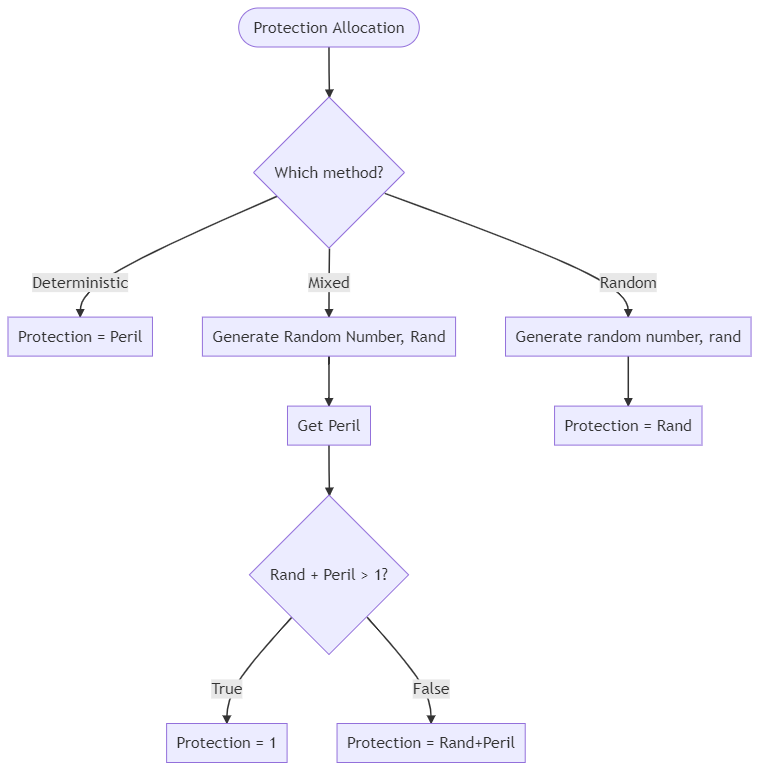
\includegraphics[width=0.75\linewidth]{assets/protection}
  \caption{Visualisation of protection allocation - this is allocated either based on proximity to infection and updated at each turn, uniformly at random at initialisation or by combination of both.}
  \label{fig:protection}
\end{figure}

We then assign an agent to each vertex. Agents can be in a number of states, such as `susceptible' (could contract), `infected' (currently has the infection and is infectious), `recovered' (previously had the infection) and `protected' (cannot contract the infection). The latter of these state is where much of our work has been focused: we have been studying the dynamics of the system with this state using the `protection ratings' of vertices. We currently assign this rating in one of three ways: purely randomly, based upon proximity to infection or a combination of the two approaches.

In Figure \ref{fig:protection}, we see that the `random' allocation currently entails assigning protection ratings uniformly at random once at the onset of the disease. These ratings do not change as the model progresses, which is in contrast to assignment based on proximity to infection where defence ratings are recalculated after each turn. Of course, this seems fairly simplistic but stands for something profound - this rating represents inclination towards self-protection, it is a reflection of simulated personality in individuals. If we wished to make this a more interesting assignment to better reflect a given population and context, we might look into assigning based on, for instance, normal or Poisson distributions. This is something that could be easily implemented based on the requirements of a given epidemic context as and when required.

Once these agents are initialised, a defensive move is made that is adapted to account for the inherent individual protection ratings. The current existing defence strategies are detailed in Figure \ref{fig:defence}. Currently, there are three main defence strategies that are deployed.

\begin{figure}[!ht]
  \centering
  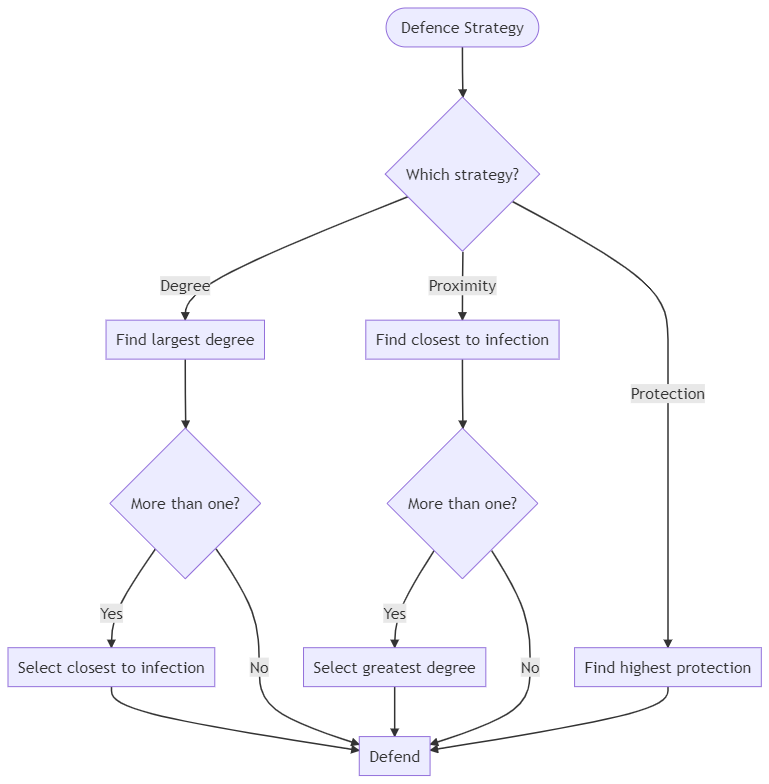
\includegraphics[width=0.75\linewidth]{assets/defence}
  \caption{Representation of three implemented defence strategies.}
  \label{fig:defence}
\end{figure}

The defence strategies are represented visually in Figure \ref{fig:defence}. These strategies are:
\begin{itemize}
	\item Defend based on highest degree, breaking ties on greatest proximity to infection;
	\item Defend based on greatest proximity to infection, break ties on highest degree; and
	\item Defend the agents who currently have the highest protection rating.
\end{itemize}
The first two of these strategies are common in classic {\scshape Firefighter} - defending based on degree is effective in fairly dense graphs and defending based on proximity to fire is effective in sparse and tree-like graphs \cite{finbow_2009}. We note that all three of these strategies are heuristic methods and are effectively all greedy algorithms, the difference-maker is what exactly each strategy is greedy about (protection rating, proximity to infection or degree).

\subsubsection{Experimental results}

To gather data about defence strategy performance, we ran multi-graph models on different graph classes and plotted the results. In Figure \ref{fig:plots}, we see the results of several experiments on Erd\"{o}s R\'{e}nyi random graphs. For each value of $p$ (the probability parameter for Erd\"{o}s R\'{e}nyi graph generation) between 0 and 1 in increments of 0.05, we generated 50 graphs on 50 vertices each. For each of these graphs, we started the contagion at each vertex of the graph in turn and stored the results of these simulations. We used this data to plot the percent of each graph infected under each defence strategy - here, the less of the graph that was infected before containment, the better. We also include the results for a purely random defence strategy for comparison, which was also run on each graph. The plots produced are box plots, with a single box for each defence strategy in each value of $p$ used. The box of each plot shows the interquartile range (from the $25^\text{th}$ to the $75^\text{th}$ percentile) with the median value indicated by a line in the box. The `whiskers' of the boxes indicate the minimum and maximum in the range, with any outliers indicated by filled-in rhombi, where relevant.

\begin{figure}[!ht] 
  \begin{centering}
    \begin{subfigure}{0.6\linewidth}
      \centering
	  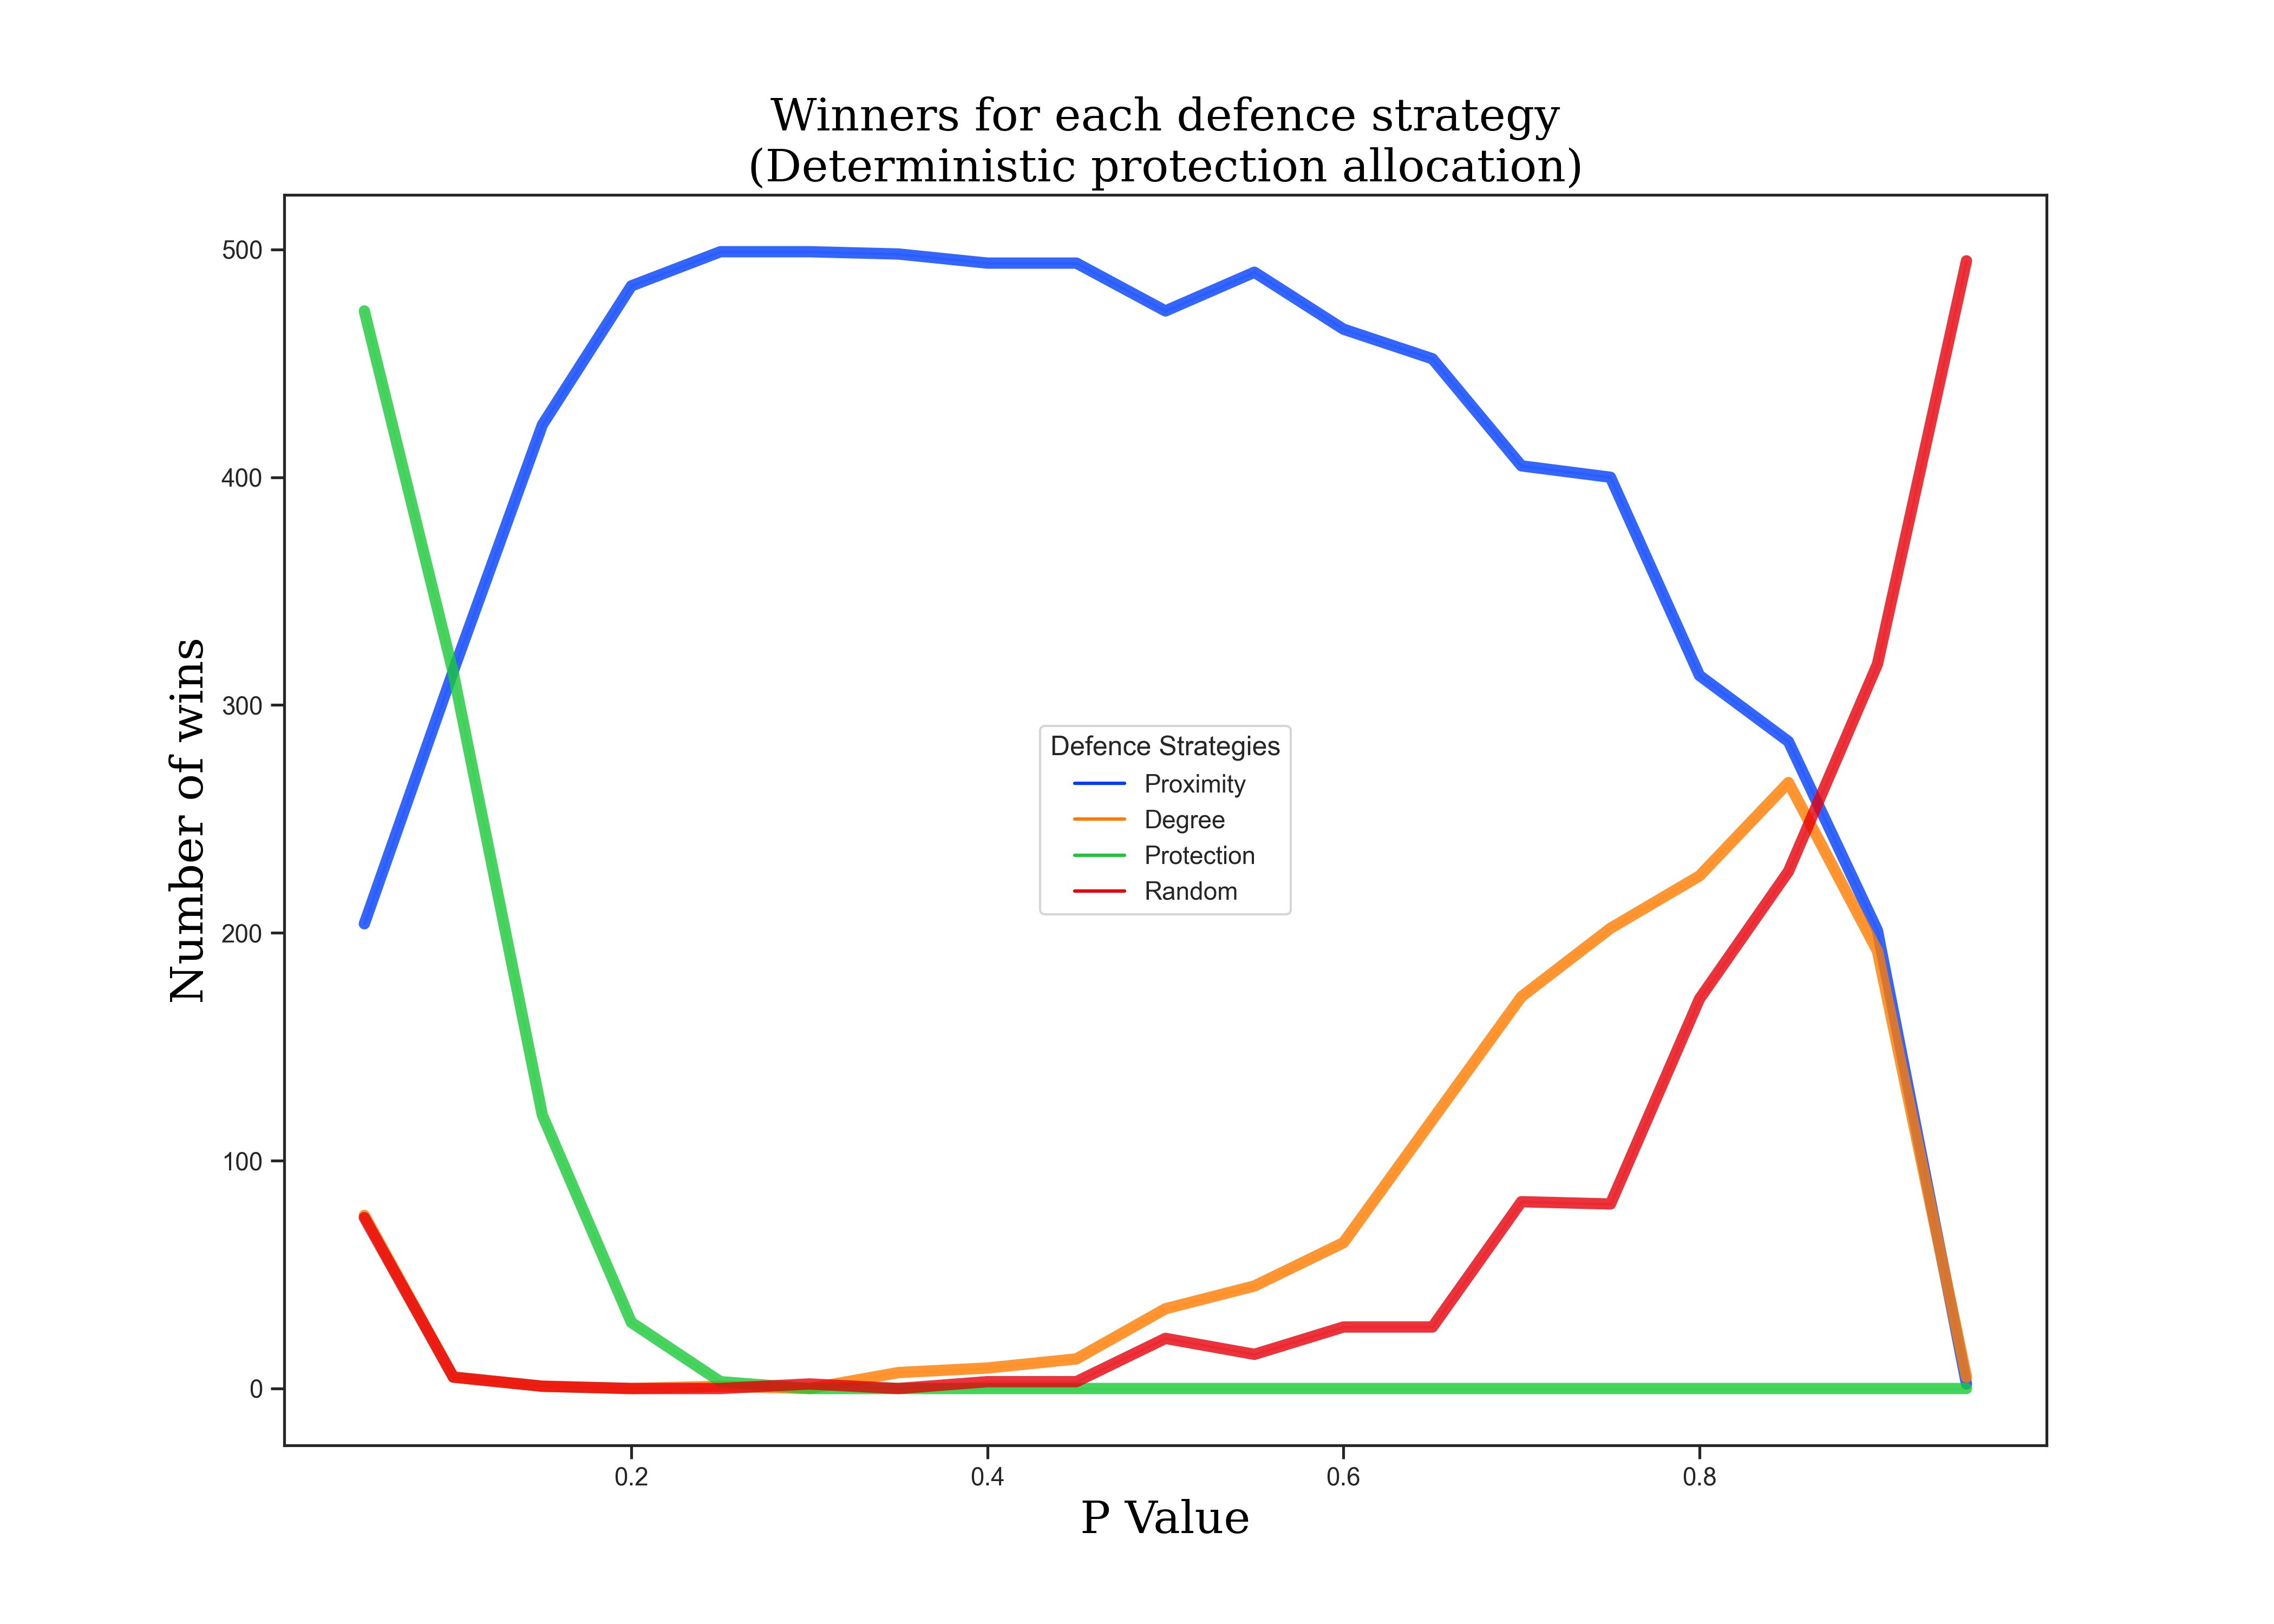
\includegraphics[width=0.91\textwidth]{charts/percent_infected/Deterministic.jpg}
	  \caption{Protection ratings are allocated based on proximity to closest infection.}
      \label{fig:det-result}
    \end{subfigure}\\
    \begin{subfigure}{0.6\linewidth}
      \centering
      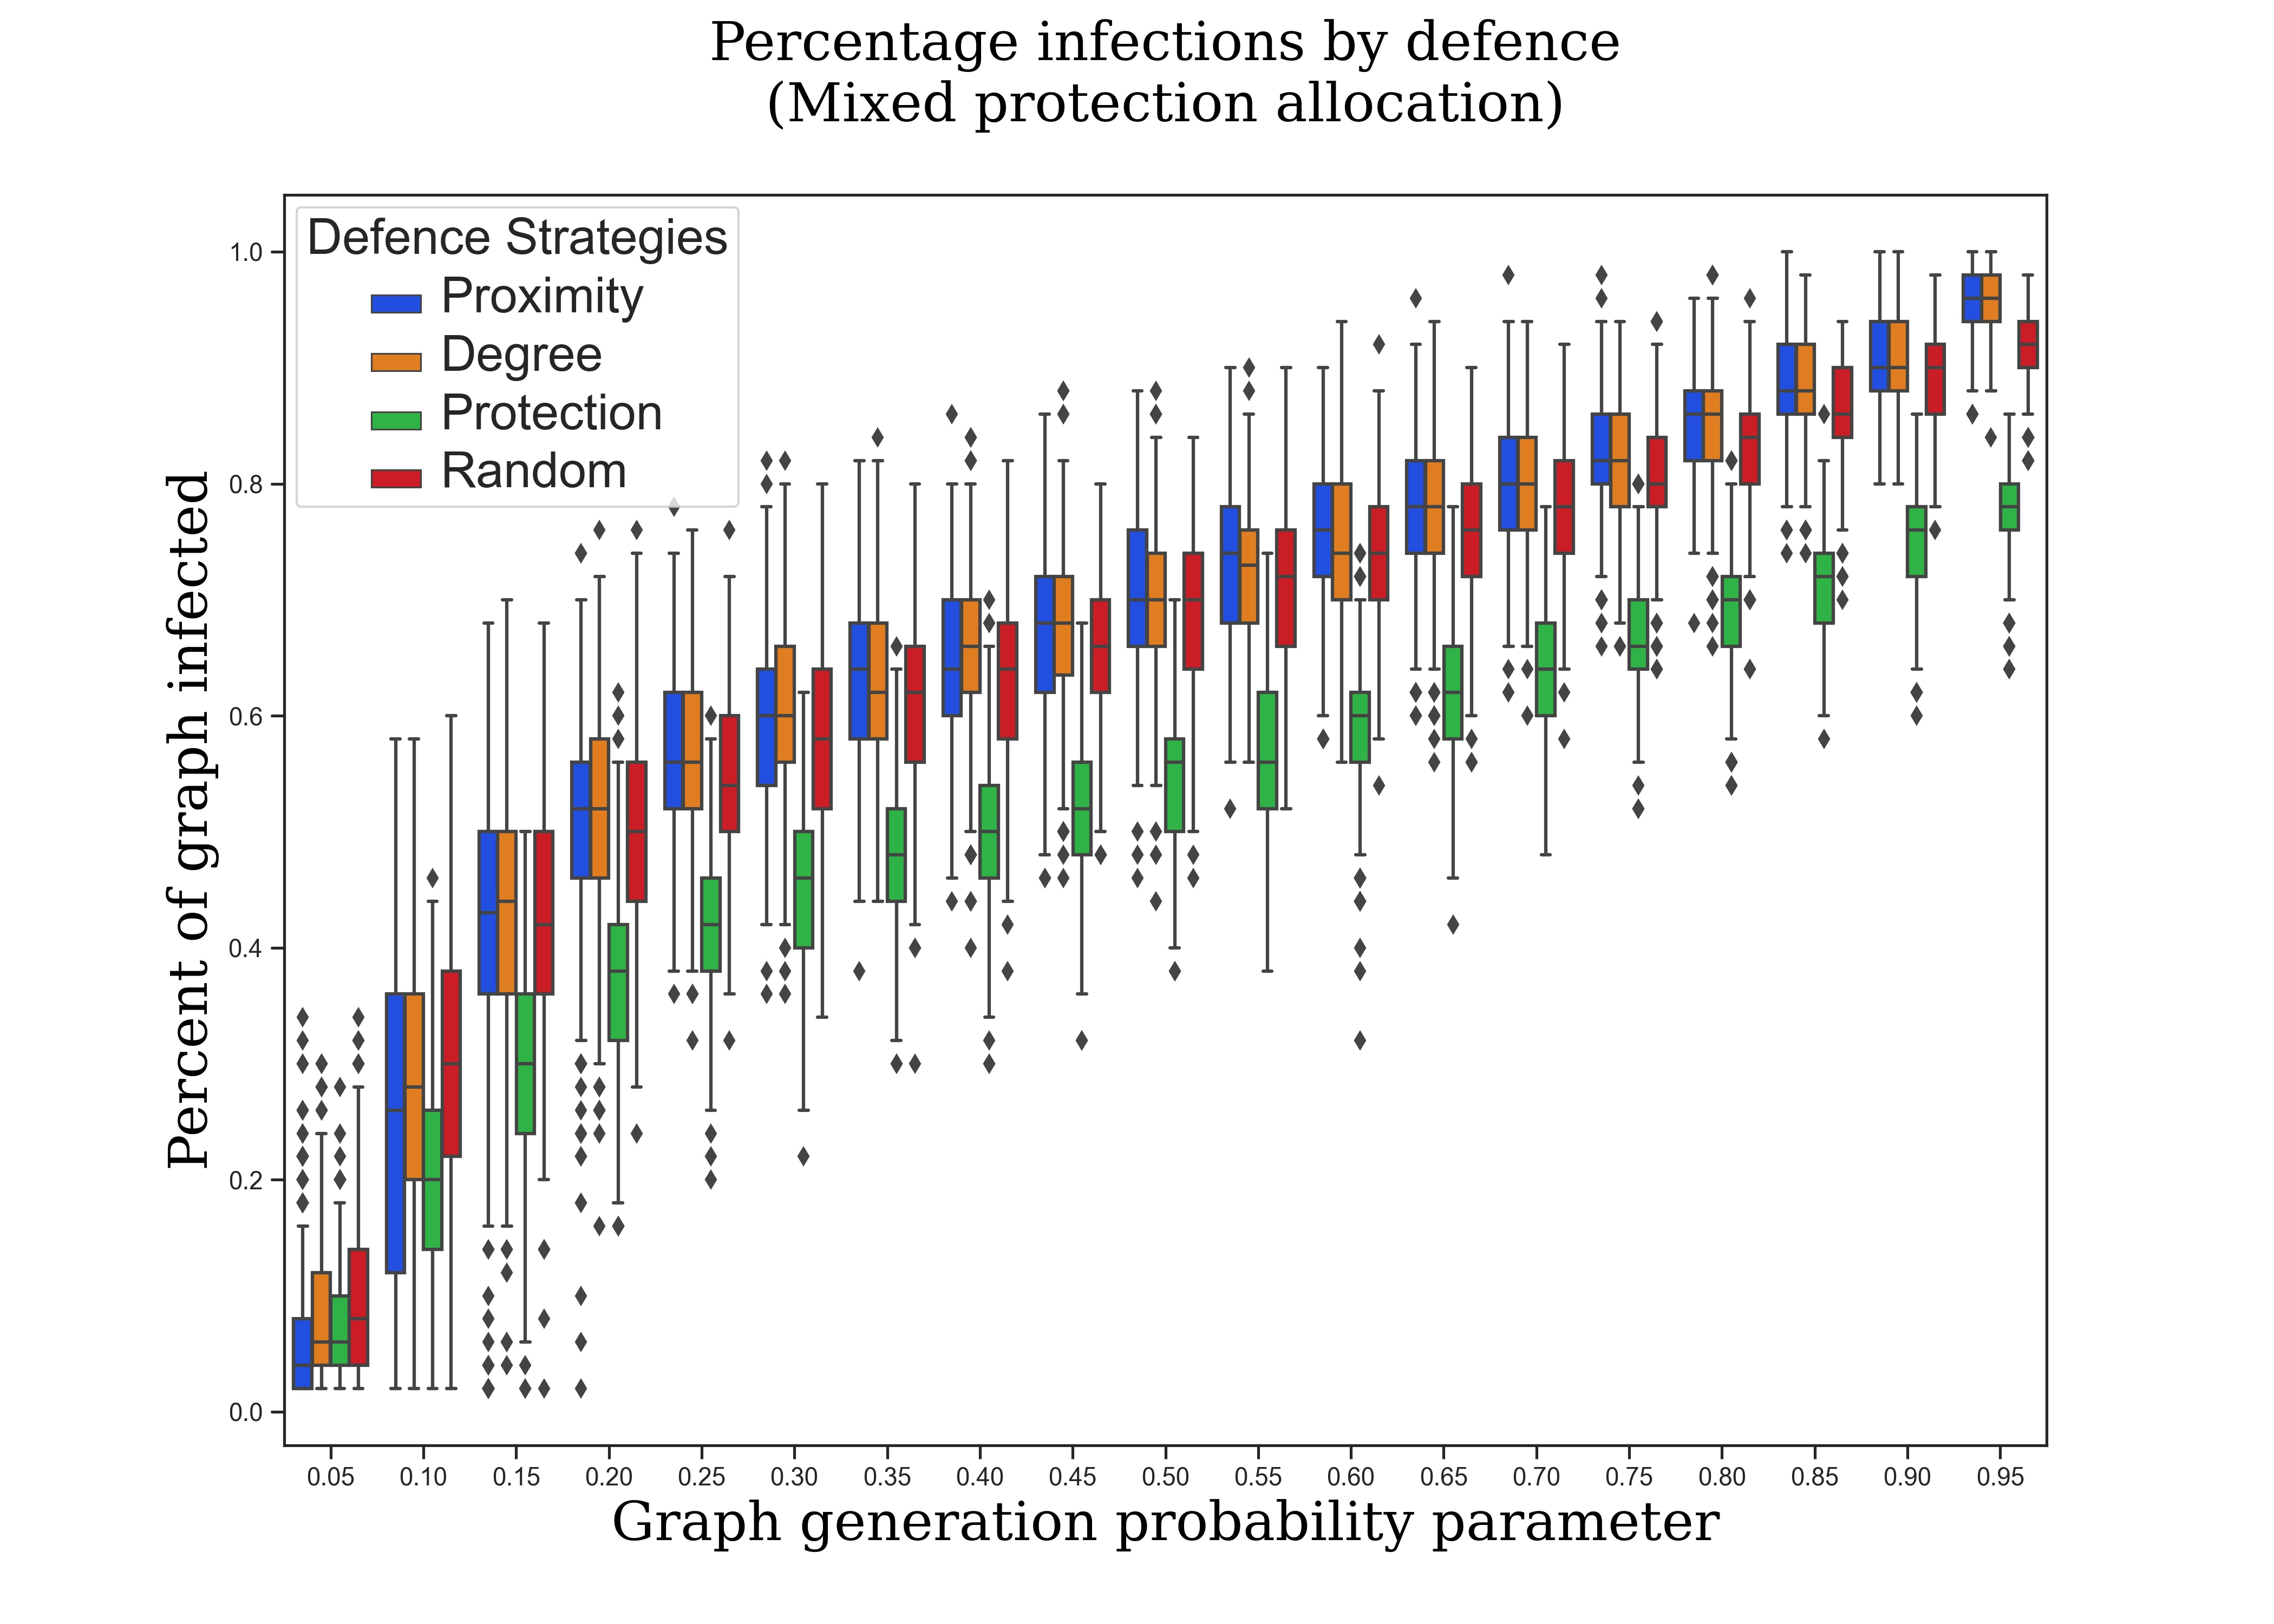
\includegraphics[width=0.91\textwidth]{charts/percent_infected/Mixed.jpg}
	  \caption{Protection ratings allocated based on a baseline random number which is increased based on proximity to closest infection.}
      \label{fig:mix-result}
    \end{subfigure}\\
    \begin{subfigure}{0.6\linewidth}
      \centering
      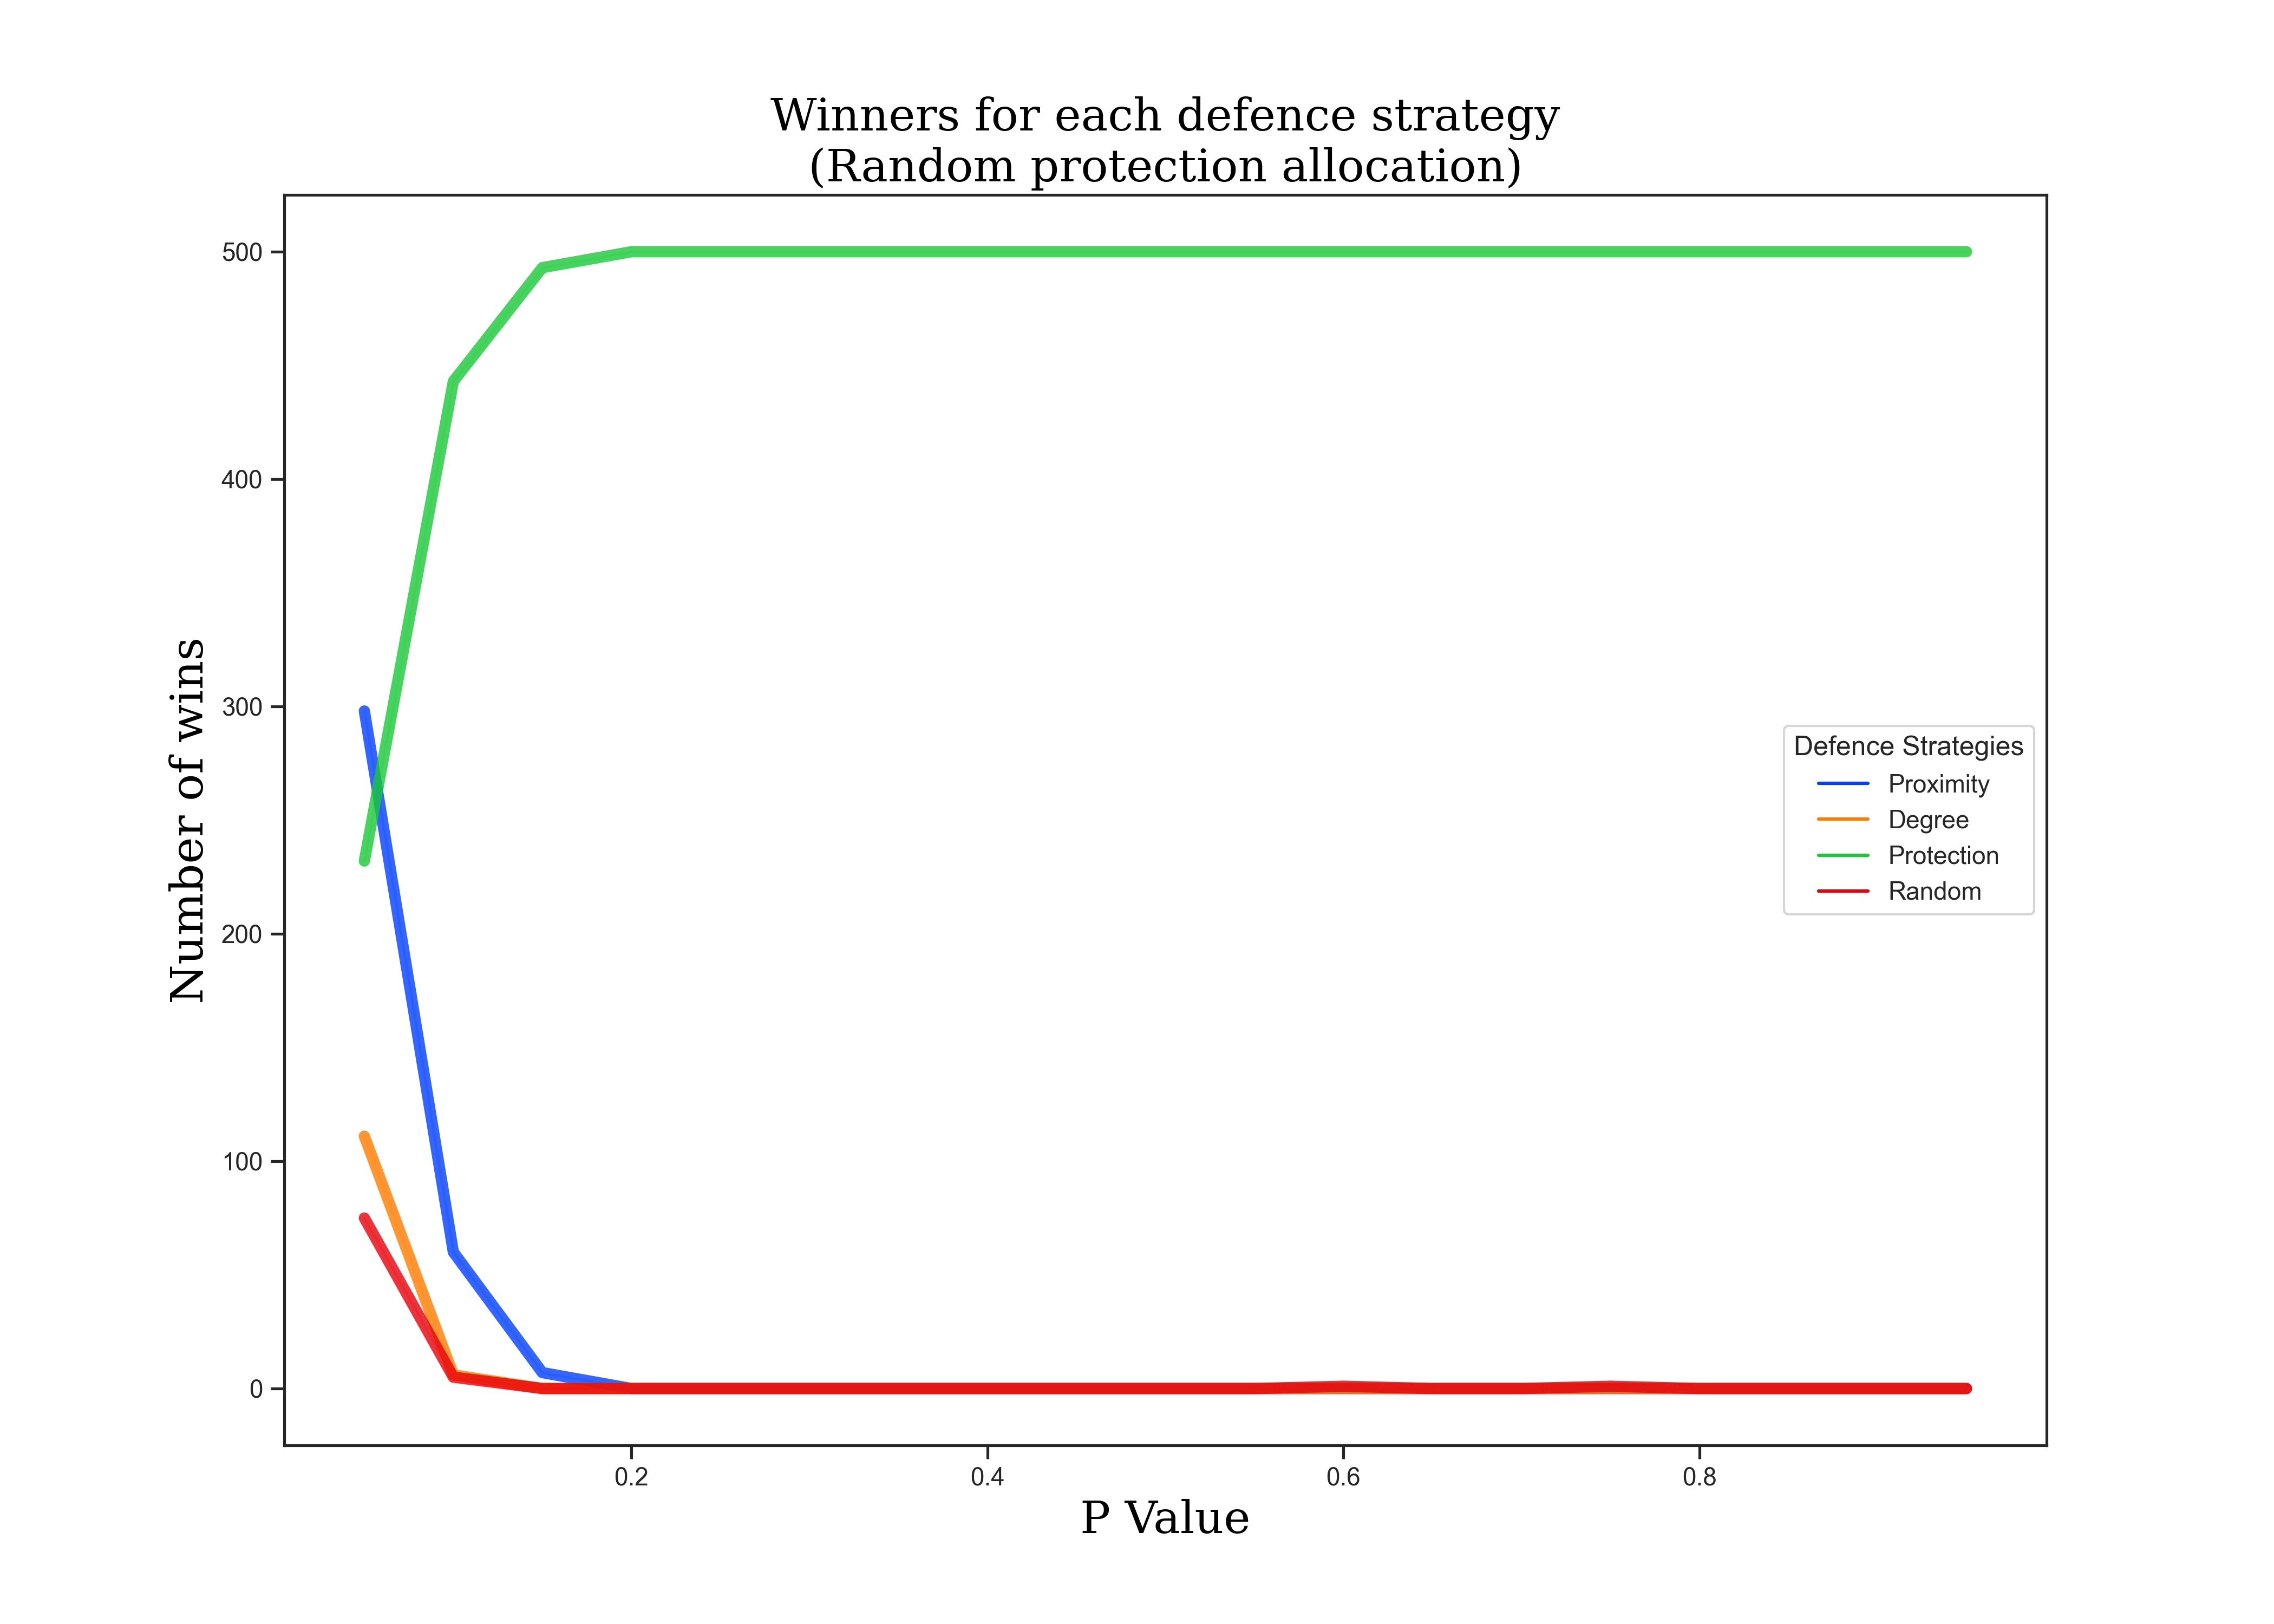
\includegraphics[width=0.91\textwidth]{charts/percent_infected/Random.jpg}
	  \caption{Protection ratings allocated uniformly at random.}
      \label{fig:ran-result}
    \end{subfigure}\\
  \end{centering}
  \caption{Charts showing a comparison of percentage of Erd\"{o}s R\'{e}nyi graphs infected when defended by three different defence strategies (and a random defence for comparison) with probability parameter $p$ varied between 0 and 1 in increments of 0.05  for three different agent protection rating allocation methods.}
  \label{fig:plots}
\end{figure}

From these plots, we can see for mixed and uniformly random protection ratings, defence based on protection rating consistently outperforms the other strategies. We can see that, when we assign internal protection purely based on proximity to infection for each agent, defence based on proximity outperforms the other strategies. We would otherwise expect this strategy to perform identically to defence based on protection: this is not the case since the protection defence does not break ties, which defence on proximity does (here, we break ties on degree).

\subsubsection{Computational Biology Conference}

On $27^{\text{th}}$ May 2021, we presented a talk on agency-oriented modelling to the First University of Glasgow Computational Biology Conference. The title of the talk was {\it Introducing features of agency into computational models of infectious disease.}
The key points of discussion were:
\begin{itemize}
\item Current computational approaches to graph models of disease
\item Extending existing graph models to better account for individual agency
\item Introducing a compartmental modelling approach
\end{itemize} 

Following this talk, we have been contacted by several students and academics interested in the work presented. For some of these individuals, we have arranged further discussion to establish potential areas for collaboration.

%%%%%

\subsection{Graph-based compartmental models}

In this section, we will detail and explain the work we have done in extending the work outlined in Section \ref{subsec:SIR-lit}. We begin by exploring the addition of a new compartmental state to a graph-based $SIR$ model and then we determine the impact this has on the total system of equations describing these models. The main focus of our work so far in this area has been to develop an algorithmic approach for the work detailed in \cite{kiss_2014} (discussed in Section \ref{subsec:SIR-lit}), which the authors of that work left as an open problem.

\subsubsection{Adding a new state to the model}

Let $\zeta_i$ be the probability that we defend individual $i$.
%This can be determined in a number of different ways and we propose that a good candidate for this would be an algorithmic approach.\footnote{That is, determine the best candidates for defence each turn and distribute some given probability across them by the expected benefit in containing the infection gained by defending each vertex.}
Similarly, let $\alpha_i$ represent the efficacy of the protection measure for individual $i$, which may decay over time and vary from person to person. Using these rates of protection and effectiveness, for fixed population size the differential equations become:
\begin{align}
\dot{\langle S_i \rangle} & = \alpha_i \langle P_i \rangle - \sum^{N}_{j=1}T_{ij} \langle S_i I_j \rangle - \zeta_i\langle S_i \rangle\\
\dot{\langle I \rangle} & =\sum^{N}_{j=1}T_{ij}\langle S_i I_j \rangle - \gamma_i \langle I \rangle \\
\dot{\langle R_i \rangle} & = \gamma_i \langle I \rangle \\
\dot{\langle P_i \rangle} & = \zeta_i \langle S_i \rangle - \alpha_i \langle P_i \rangle.
\end{align} 
%Accounting for vital dynamics, with a birth and death rate (for simplicity) of $\mu$, these equations are:
%\begin{align}
%\dot{\langle S_i \rangle} & = \alpha_i \langle P_i \rangle - \sum^{N}_{j=1}T_{ij} \langle S_i I_j \rangle + \mu N - \mu \langle S_i \rangle - \zeta_i\langle S_i \rangle\\
%\dot{\langle I \rangle} & =\sum^{N}_{j=1}T_{ij}\langle S_i I_j \rangle - \gamma_i \langle I \rangle - \mu \langle I_i \rangle\\
%\dot{\langle R_i \rangle} & = \gamma_i \langle I \rangle + \mu \langle R_i \rangle\\
%\dot{\langle P_i \rangle} & = \zeta_i \langle S_i \rangle - \alpha_i \langle P_i \rangle - \mu \langle P_i \rangle.
%\end{align}

\subsubsection{Results for total system of equations}

As an example, we consider the `triangle network' - a loop of three nodes. The equations required to precisely express the system $SIR$ dynamics of this network are as follows \cite{kiss_2014}:
\begin{align}
\text{6 singles: } & \dot{\langle S_1 \rangle}, \dot{\langle S_2 \rangle}, \dot{\langle S_3 \rangle}, \dot{\langle I_1 \rangle}, \dot{\langle I_2 \rangle}, \dot{\langle I_3 \rangle}.\label{eq:SIRsingle}\\
\text{6 doubles: } & \dot{\langle S_1 I_2 \rangle},\dot{\langle I_1 S_2 \rangle}, \dot{\langle S_1 I_3 \rangle}, \dot{\langle I_1 S_3 \rangle}, \dot{\langle S_2 I_3\rangle}, \dot{\langle I_2 S_3 \rangle}.\label{eq:SIRdouble}\\
\text{6 triples: } & \dot{\langle S_1 I_2 I_3 \rangle}, \dot{\langle S_1 I_2 S_3 \rangle}, \dot{\langle S_1 S_2 I_3 \rangle}, \dot{\langle I_1 S_2 S_3 \rangle}, \dot{\langle I_1 I_2 S_3 \rangle}, \dot{\langle I_1 S_2 I_3 \rangle}. \label{eq:SIRtriple}
\end{align}
Now, using the equations for the $SIRP$ model, we have the following equation requirements:
\begin{align*}
\text{9 singles: (} \ref{eq:SIRsingle} \text{) and } & \dot{\langle P_1 \rangle}, \dot{\langle P_2 \rangle}, \dot{\langle P_3 \rangle}.\\
\text{18 doubles: (} \ref{eq:SIRdouble} \text{) and }& \dot{\langle S_1 P_2 \rangle},\dot{\langle P_1 S_2 \rangle}, \dot{\langle I_1 P_2 \rangle}, \dot{\langle P_1 I_2 \rangle}, \dot{\langle S_1 P_3\rangle}, \dot{\langle P_1 S_3 \rangle},\\ & \dot{\langle I_1 P_3 \rangle}, \dot{\langle P_1 I_3 \rangle}, \dot{\langle S_2 P_3 \rangle}, \dot{\langle P_2 S_3 \rangle}, \dot{\langle I_2 P_3 \rangle}, \dot{\langle P_2 I_3 \rangle}. \\
\text{24 triples: (} \ref{eq:SIRtriple} \text{) and } & \dot{\langle S_1 S_2 P_3 \rangle}, \dot{\langle S_1 P_2 S_3 \rangle}, \dot{\langle S_1 I_2 P_3\rangle}, \dot{\langle S_1 P_2 I_3 \rangle}, \dot{\langle S_1 P_2 P_3\rangle}, \dot{\langle I_1 S_2 P_3 \rangle},\\
&  \dot{\langle I_1 P_2 S_3 \rangle}, \dot{\langle I_1 I_2 P_3 \rangle}, \dot{\langle I_1 P_2 I_3 \rangle}, \dot{\langle I_1 P_2 P_2 \rangle},  \dot{\langle P_1 S_2 S_3 \rangle}, \dot{\langle P_1 S_2 I_3 \rangle},\\
&  \dot{\langle P_1 I_2 S_3 \rangle}, \dot{\langle P_1 I_2 I_3 \rangle}, \dot{\langle P_1 P_2 I_3 \rangle},  \dot{\langle P_1 P_2 S_3 \rangle}, \dot{\langle P_1 S_2 P_3 \rangle},  \dot{\langle P_1 I_2 P_3\rangle}.
\end{align*}

Note that the reason we dispense with the cases of all three vertices being in the same state is that this would not result in any dynamics - no vertices would ever change state in this case. 

\subsubsection{Implementation}
\label{subsubsec:implementation}

We have been working on an implementation of the above work in equations generation. Our goal is to produce code that can accept a particular graph, for instance as a CSV file, and determine the number of equations that could be required to fully describe a compartmental model (for instance, $SIR$ or $SIRP$) on that graph. This could be by providing upper and lower bounds if the exact graph structure is unknown, or by providing the exact number of equations if the graph is known. With this information, the user can request the software returns the full list of differential equations that exactly describe the epidemic dynamics using an algorithmic approach to generation.

\subsection{Uses of Percolation in The Firefighter Problem}
\label{subsec:perc-fire}

We have identified two main avenues that we would like to explore further regarding the use of Percolation Theory in {\scshape Firefighter}: the firefighter may use percolation in order to defend the graph, or the fire might spread with percolation probability $p$. We will now discuss these two possible avenues and how we hope to use them in our research.

%\begin{figure}[ht]
%	\centering
%		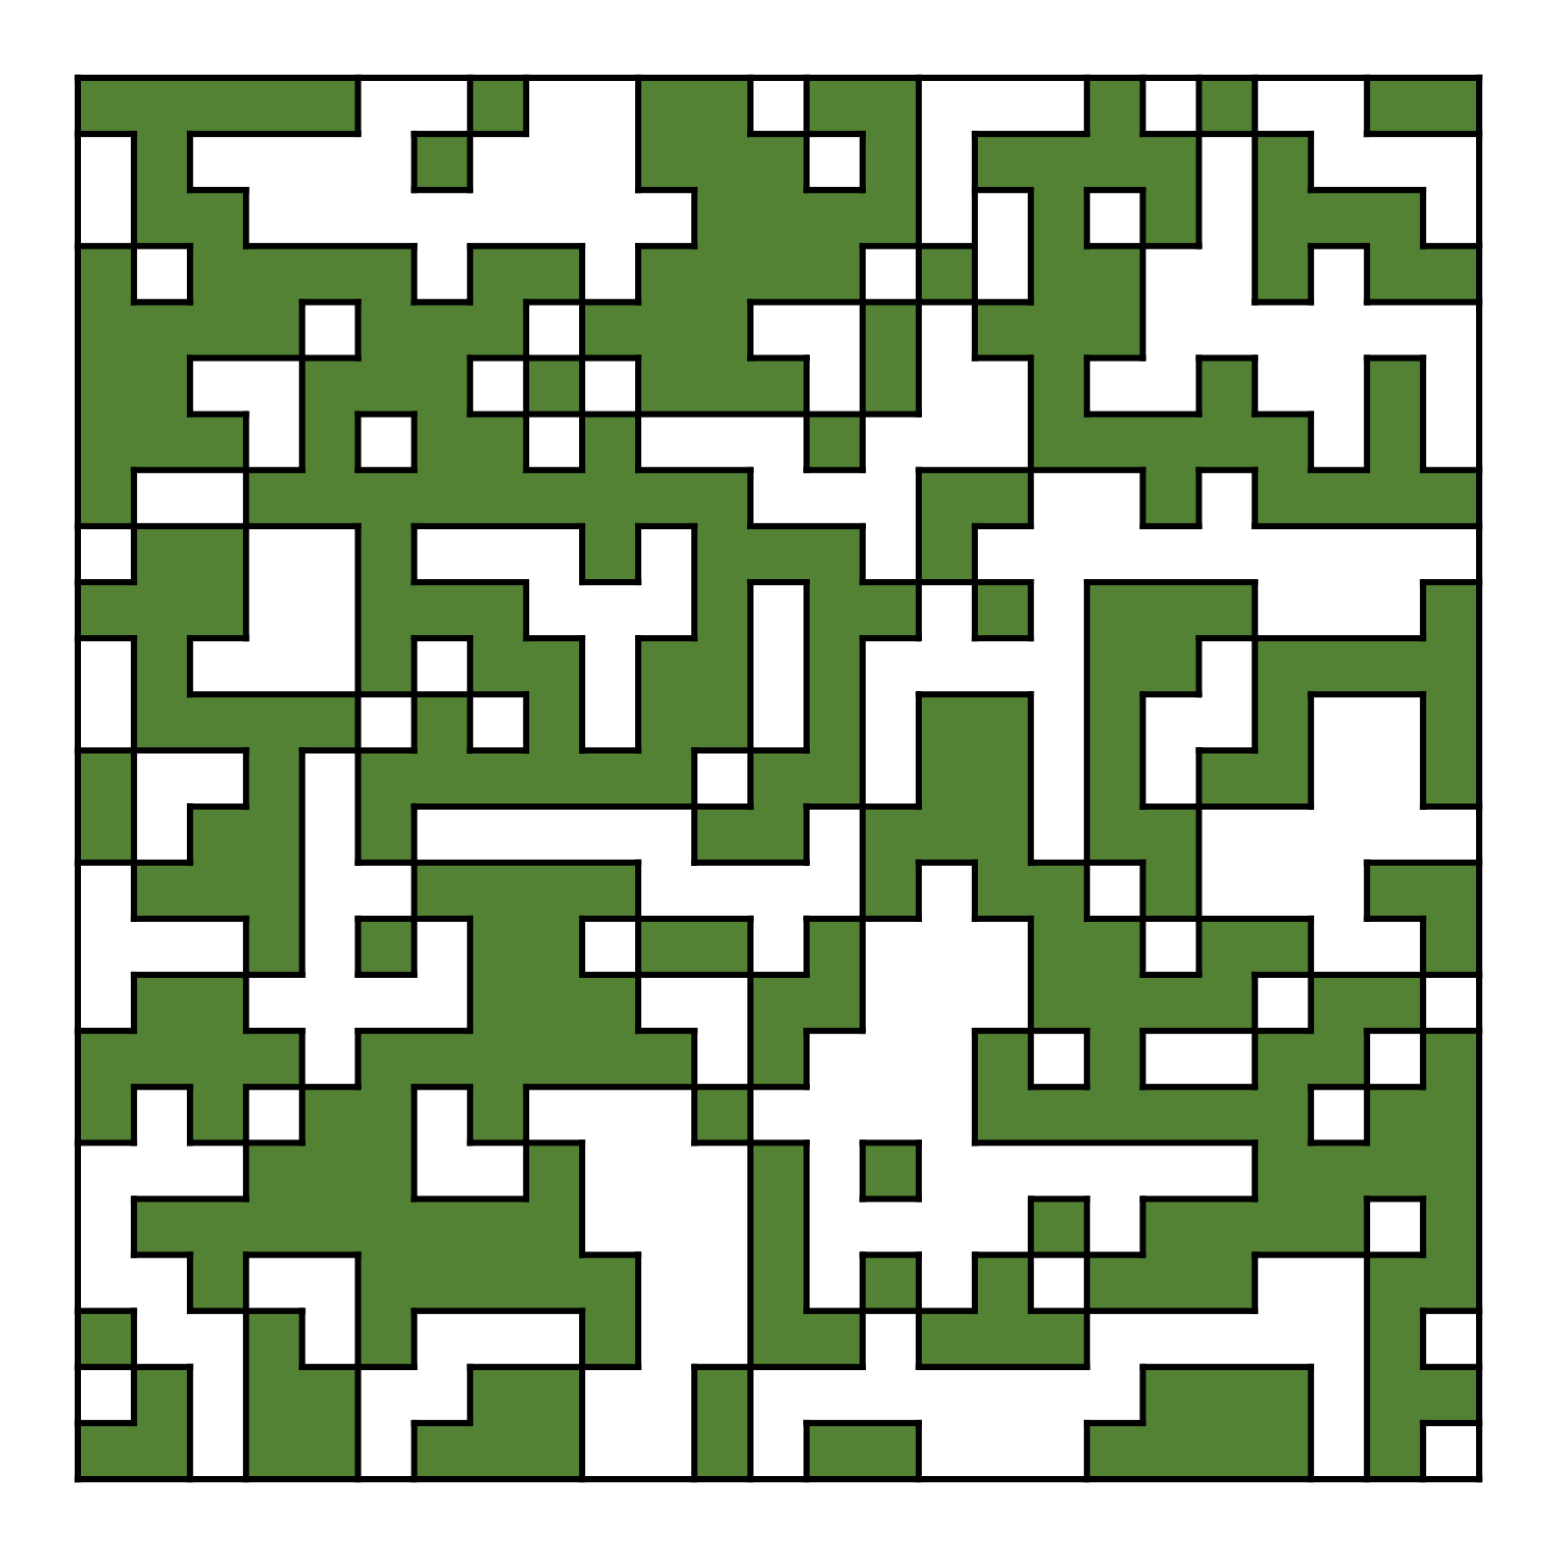
\includegraphics[width=0.3\linewidth]{firebreak/25x25/25x25}
%	\caption{A 4-regular $(25\times25)$ graph, percolated with probability $p=2/3$.}
%	\label{fig:largeperc}
%\end{figure}

%%%%%%%%%%

\subsubsection{Better than random}

One potential use of percolation is a baseline test. In most scenarios, a method for obtaining defence strategies should be at least as effective as a random defence sequence. We could find such a random sequence by allowing the firefighter to defend in a percolation-like strategy for comparitive purposes. Consider a sequence of vertices in graph $G$, written as $d_1, d_2,\dots, d_t$. An optimal defence sequence could be found using integer programming as provided by Finbow and MacGillivray \cite{finbow_2009}:
\begin{equation*}
	\begin{array}{ll@{}ll}
\text{Maximise}  & \displaystyle \sum\limits_{v\in V(G)} d_v w(v) &\text{~for each level~} i\\
\text{subject to}& d_v + \displaystyle\sum\limits_{\text{level}(v)=i} d_v \leq 1  &\text{~for each level~} i\\
				 & d_v + \displaystyle\sum\limits_{u\succ v}  d_u \leq 1  &\text{~for every outer vertex~} v \text{~of~} T,\\
                 &d_{v} \in \{0,1\}. &
	\end{array}
\end{equation*}
where $u\succ v$ indicates that $u$ is an ancestor of $v$. The optimal strategies provided for different classes and densities of graphs here will provide an upper bound (which may indeed be impossible to attain in some cases) for success of a given strategy. We can find a lower bound using percolation, and so we have a range of success values as a starting point: if some strategy is better than random percolation, then it is worth considering, but below the particular expected optimal solution from integer programming and we can, in principle, improve or find a better strategy.

We conjecture that, at the lowest graph densities, the random strategy will be close to the optimal strategy and thus finding an improvement is at once difficult and lacking in great utility. At the very highest graph densities, random strategies will have a very low expected best-case scenario but so will most strategies, since the constraint on the firefighter that they have only one vertex to save per turn does not go as far towards fire containment per turn compared to sparser graphs.

\subsubsection{Reproduction rate}

We might also consider the fire spread being determined by percolation (rather than the firefighter's defence sequence). Diseases, when there is a large enough sample size, have a basic reproduction rate associated with them, denoted $R_0$: for instance, measles has a basic reproduction rate $12\leq R_0 \leq 18$ \cite{guerra_2017} and the Influenza strain responsible for the 1918 pandemic has a basic reproduction rate of $1.4 \leq R_0 \leq 2.8$ \cite{ferguson_2006}. These baseline, theoretical values can be implemented as an internal probability to a propagating fire: to formulate a stochastic version of {\scshape Firedfighter}, we let the fire propagate with some probability (which could be determined by reproduction rate of a real infectious disease) in a percolation-like process and examine the change to optimal defence.

Where we wish to consider vertices as individuals and edges as the connections between them, percolation may give us a more useful model for disease spread when we do not assume the population is well mixed and instead introduce probability functions to correspond to the likelihood one vertex is connected to another.

%\subsubsection{Irregular population density}
%
%A great deal of the literature surrounding {\scshape Firefighter} assumes a regular graph - that is, in the context of disease we assume a well-mixed population where everyone has equal probability of coming into contact with their neighbours. Of course, this is a simplification of reality: some individuals are very well connected and have lots of contact with others, and others have significantly less contact. In the context of a forest fire, the density of a forest is naturally irregular and there is a probability in the unit interval that fire can spread between two trees depending on their proximity (among other factors): an example of this can be seen in figure \ref{fig:largeperc}. Thus, percolation on regular grids to more closely resemble populations or forest density could lead to far more useful and realistic modelling results. If we start models on graphs which have been percolated with some given probability, we can ensure the model better resembles the density and irregularity of a natural population. 
%
%\begin{figure}[!ht] 
%\begin{centering}
%  \begin{subfigure}{0.4\linewidth}
%    \centering
%    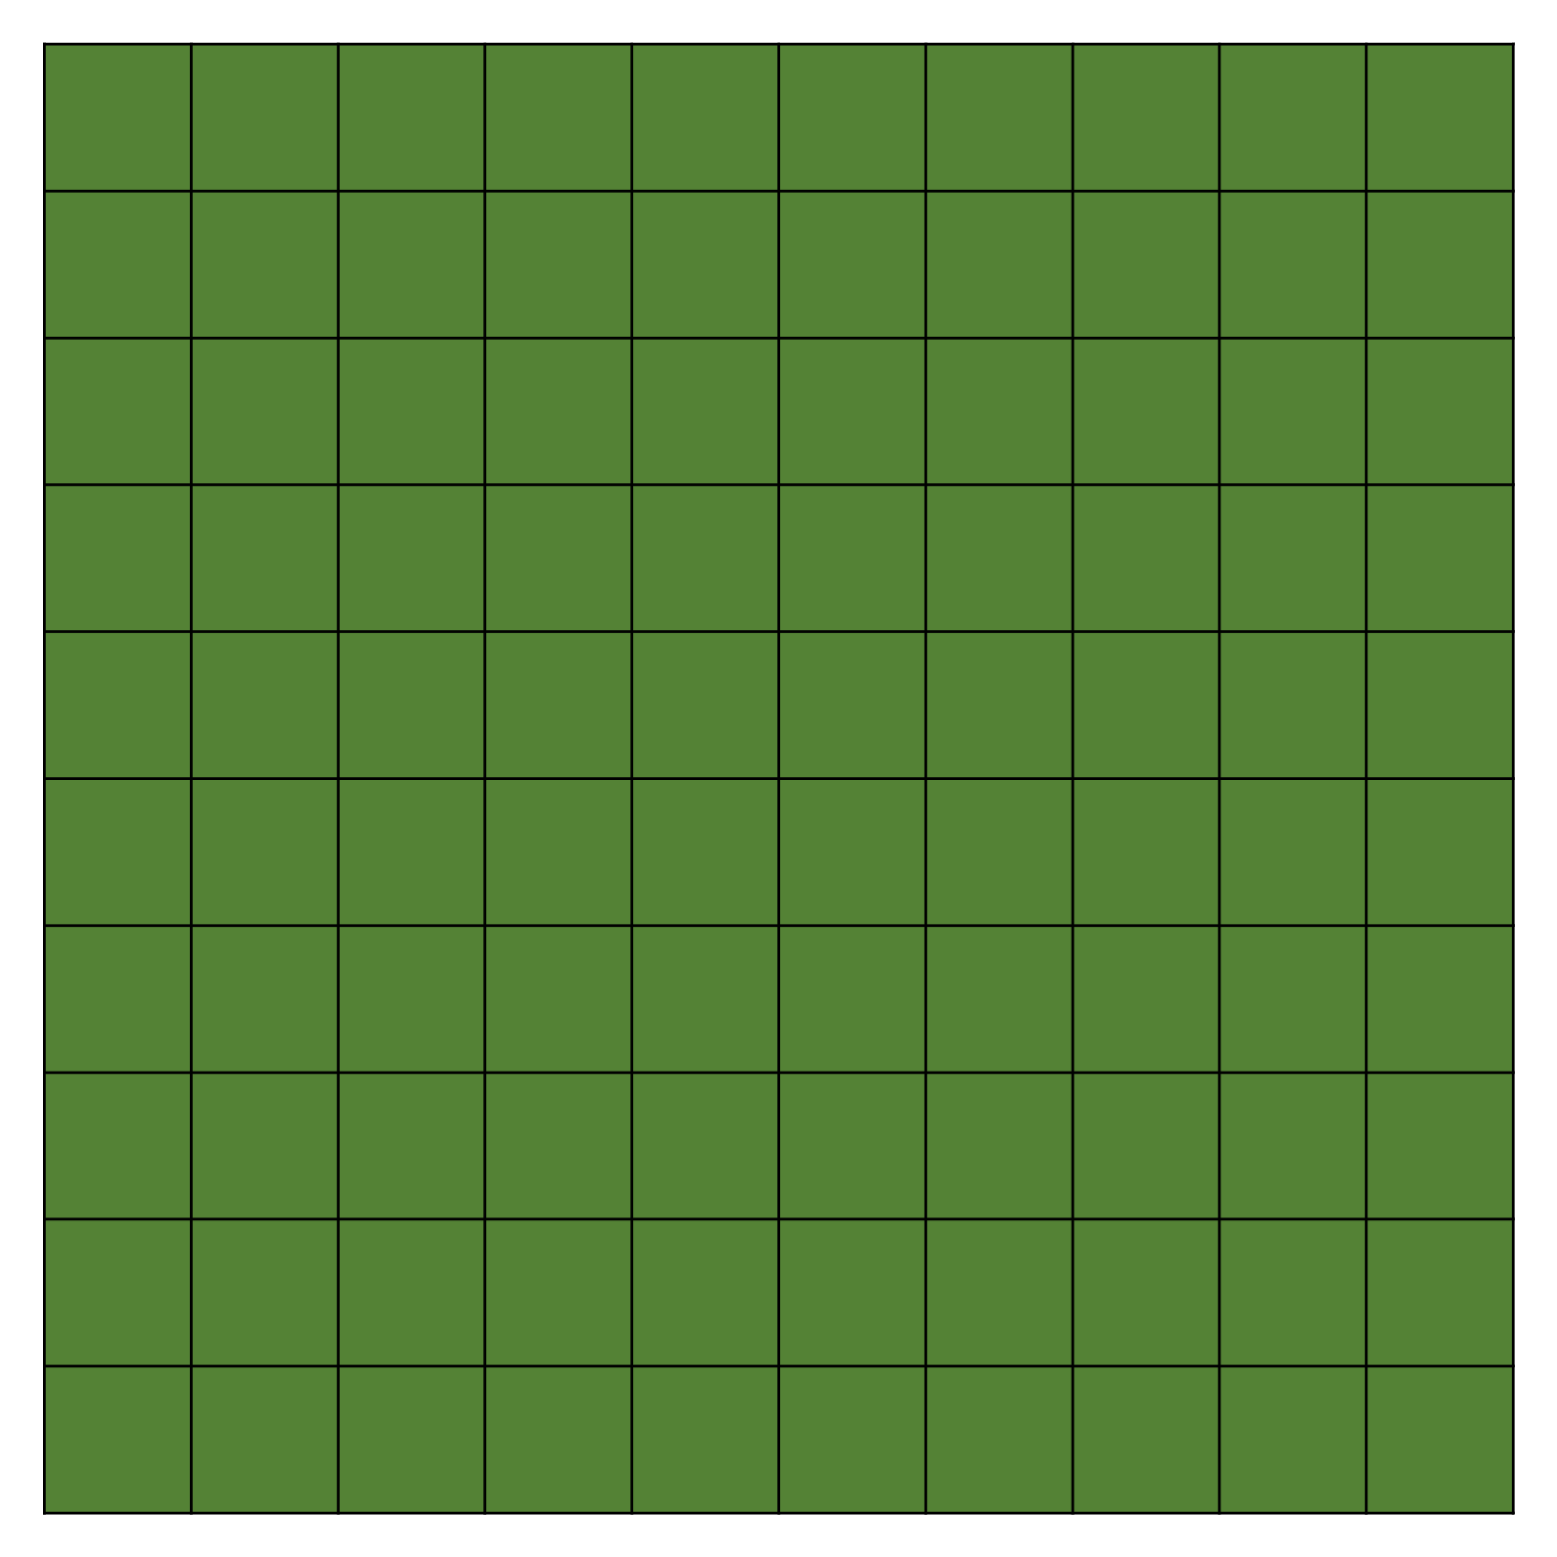
\includegraphics[width=0.4\linewidth]{firebreak/original} 
%    \caption{Initial regular graph} 
%    \label{fig:original} 
%    \vspace{4ex}
%  \end{subfigure}%% 
%  \begin{subfigure}{0.4\linewidth}
%    \centering
%    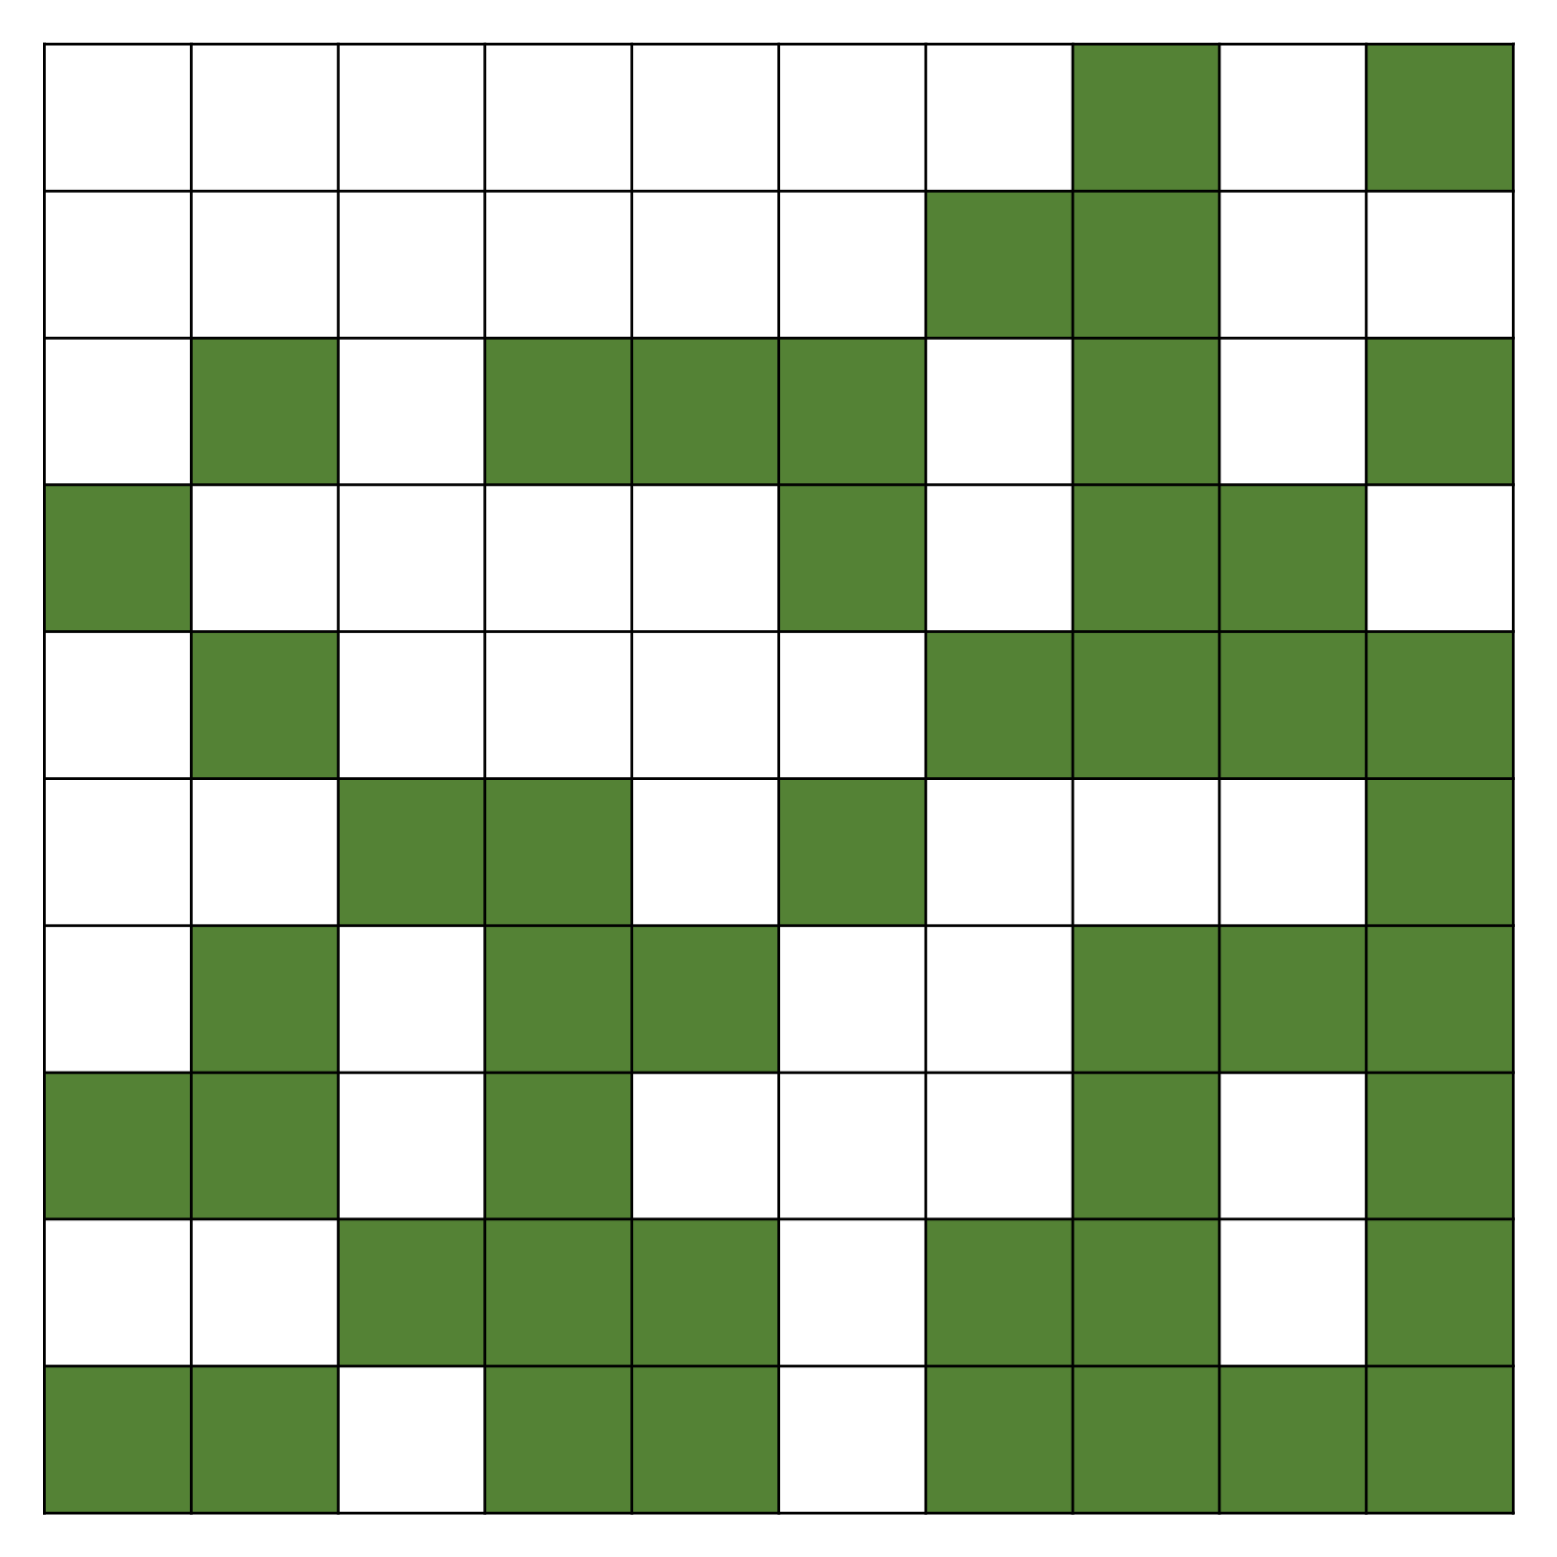
\includegraphics[width=0.4\linewidth]{firebreak/afterperc} 
%    \caption{Graph after percolation ($p=1/2$)} 
%    \label{fig:afterperc} 
%    \vspace{4ex}
%  \end{subfigure} 
%  \begin{subfigure}{0.4\linewidth}
%    \centering
%    \includegraphics[width=0.4\linewidth]{firebreak/outbreak} 
%    \caption{Initial outbreak ($t=0$)} 
%    \label{fig:outbreak} 
%  \end{subfigure}%%
%  \begin{subfigure}{0.4\linewidth}
%    \centering
%    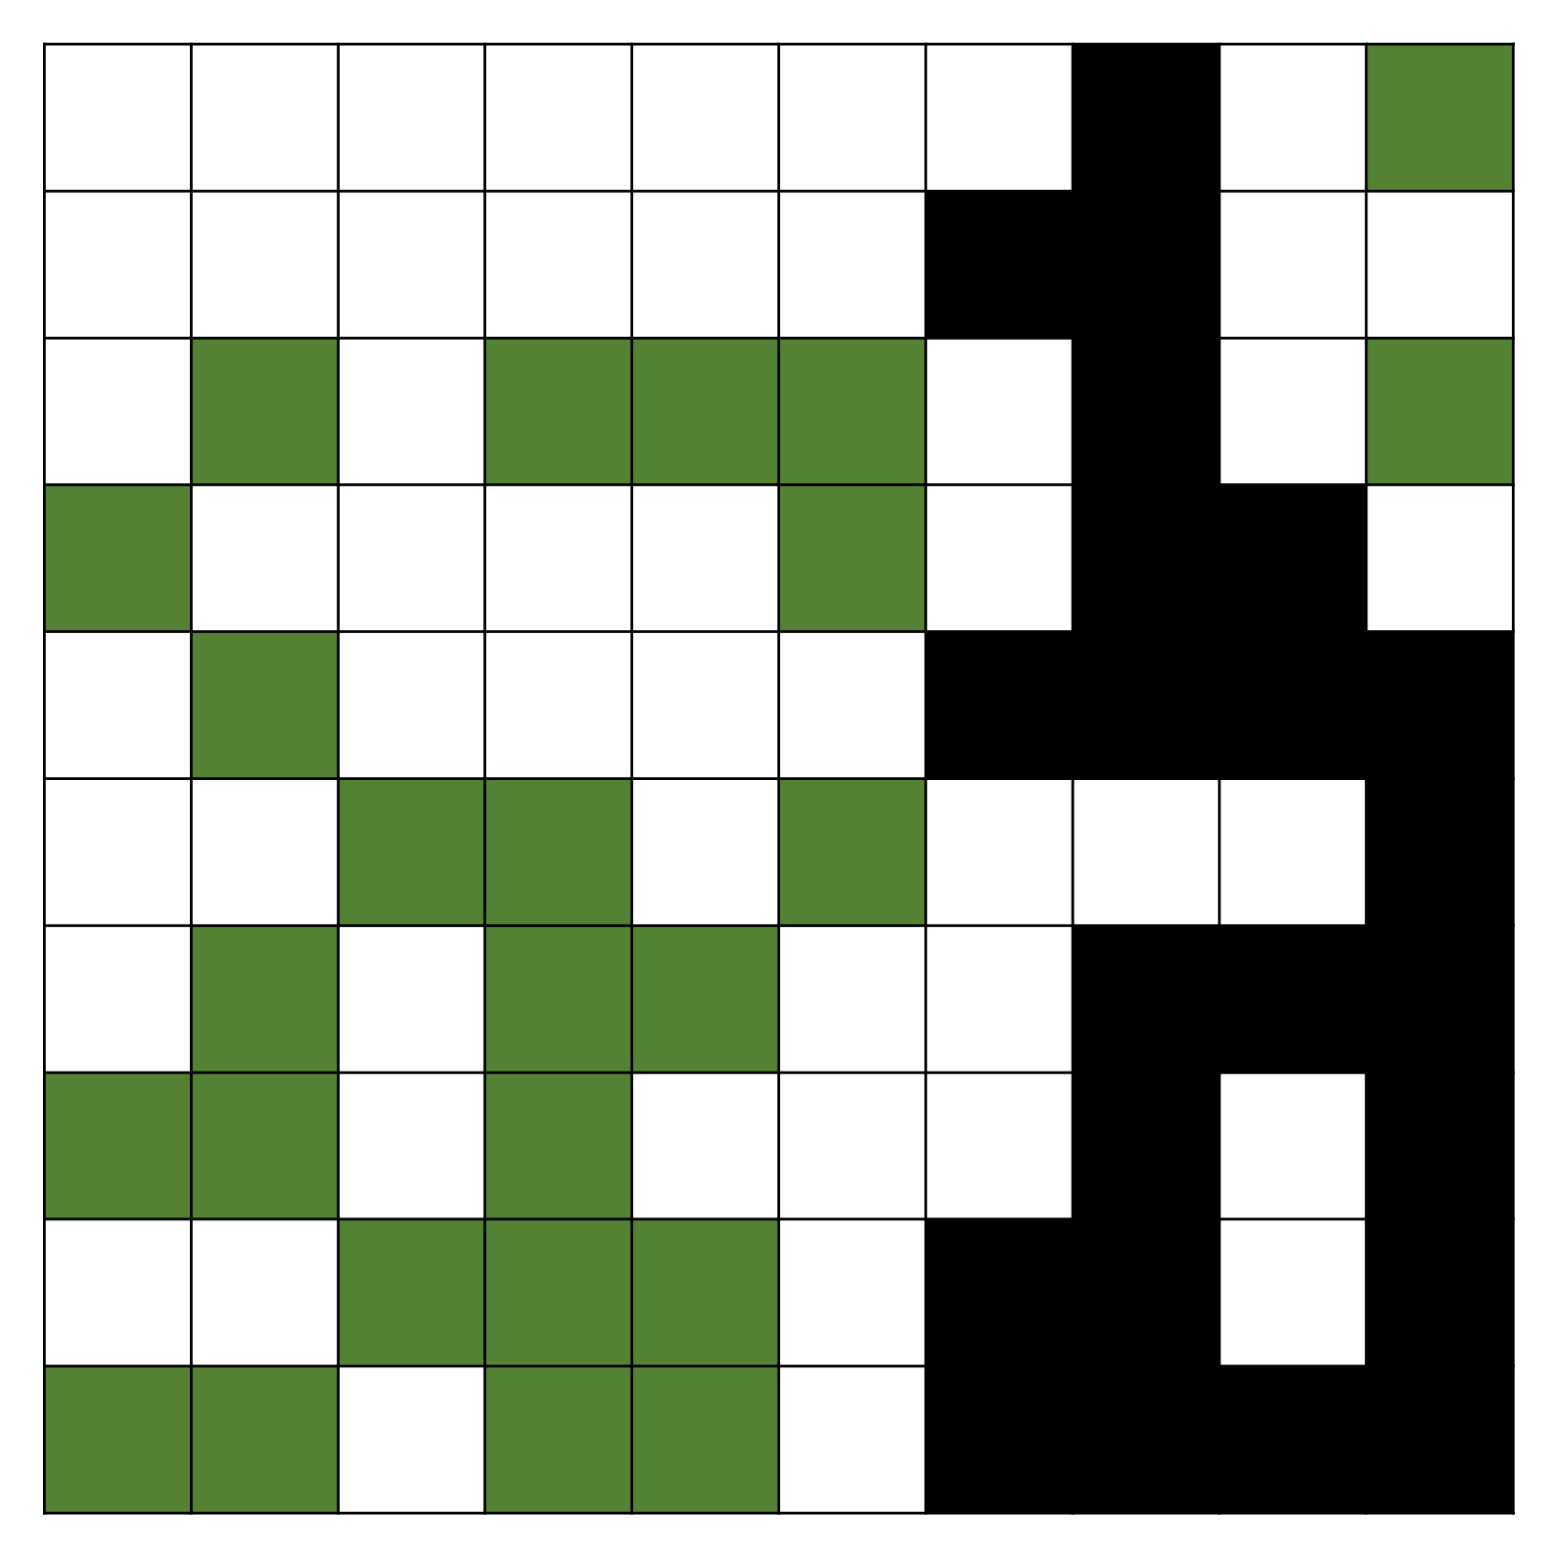
\includegraphics[width=0.4\linewidth]{firebreak/afteroutbreak} 
%    \caption{End of outbreak ($t=12$)} 
%    \label{fig:end} 
%  \end{subfigure} 
%  \caption{Outbreak of fire on a percolated graph}
%  \label{fig:percolated_graph} 
%  \end{centering}
%\end{figure}
%
%To illustrate this idea, we will consider a similar problem to {\scshape Firefighter}, called The Firebreak Problem or simply {\scshape Firebreak}. Rather than have a firefighter reactively combatting the fire on each turn, we begin with an allocated amount of funding with which to mitigate the expected damage of the fire, and spend all of that before the fire begins. Generally, this means we have a number of edges to remove (trees to cut down or place a barrier in between) before the fire begins. Figure \ref{fig:percolated_graph} depicts the use of percolation on a graph to model a forest fire. We can see that the model would have little utility if we began the outbreak on the graph in \ref{fig:original} (all of the graph would be burnt), but percolation has made this a more instructive and realistic model in figure \ref{fig:afterperc}. We can see where the fire has spread in \ref{fig:end}, and we can see where - if we had a finite amount of resources - we must focus our efforts and funding in introducing a firebreak.
%
%\begin{figure}[ht] 
%\begin{centering}
%  \begin{subfigure}{0.4\linewidth}
%    \centering
%    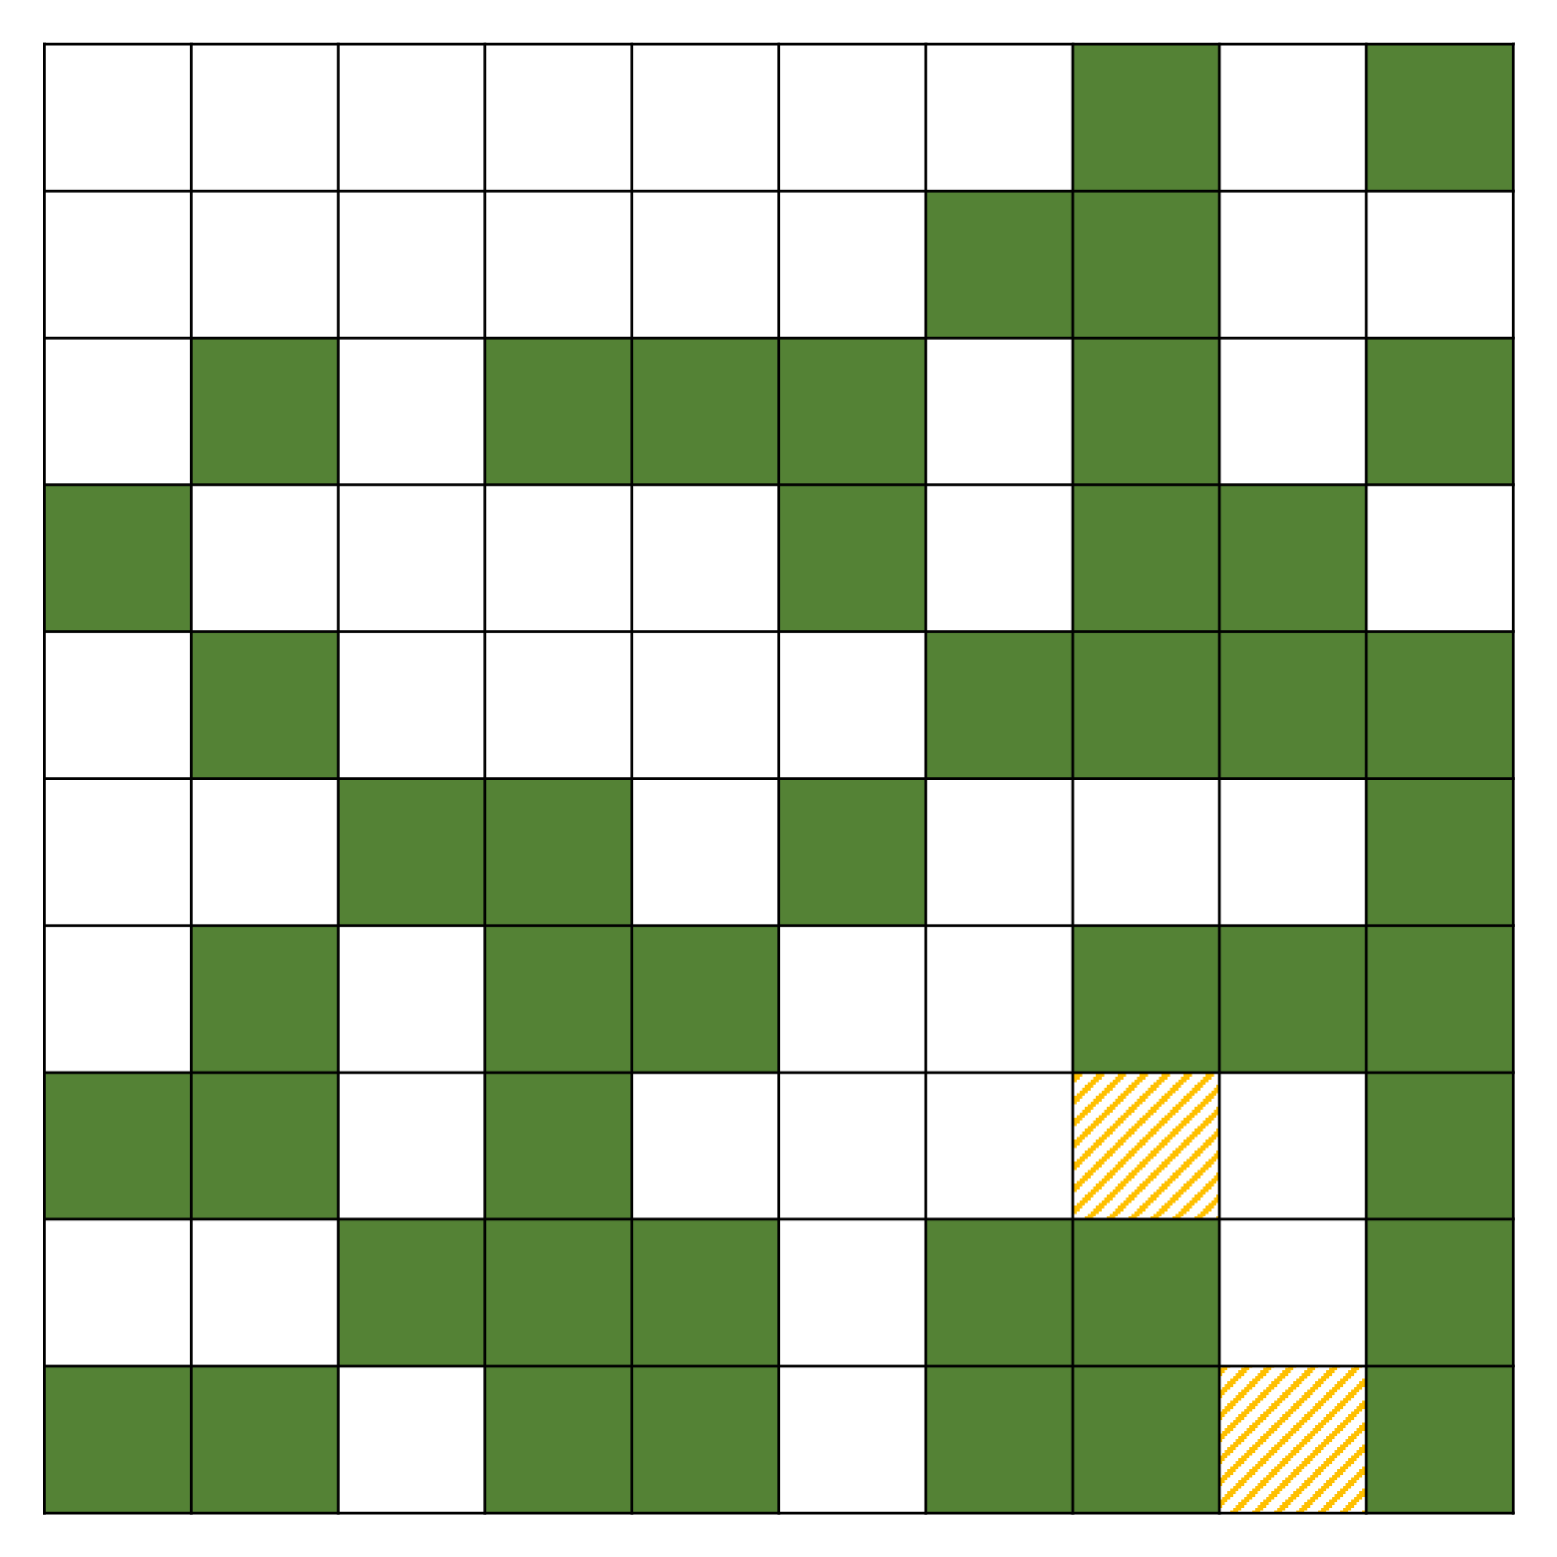
\includegraphics[width=0.4\linewidth]{firebreak/defended/defended} 
%    \caption{Position of Firebreak (in yellow)} 
%    \label{fig:defended} 
%    %\vspace{4ex}
%  \end{subfigure}%% 
%  \begin{subfigure}{0.4\linewidth}
%    \centering
%    \includegraphics[width=0.4\linewidth]{firebreak/defended/outbreak} 
%    \caption{Fire onset with firebreak ($t=0$)} 
%    \label{fig:afterperc_break} 
%    %\vspace{4ex}
%  \end{subfigure}\\[1ex] 
%  \begin{subfigure}{0.4\linewidth}
%    \centering
%    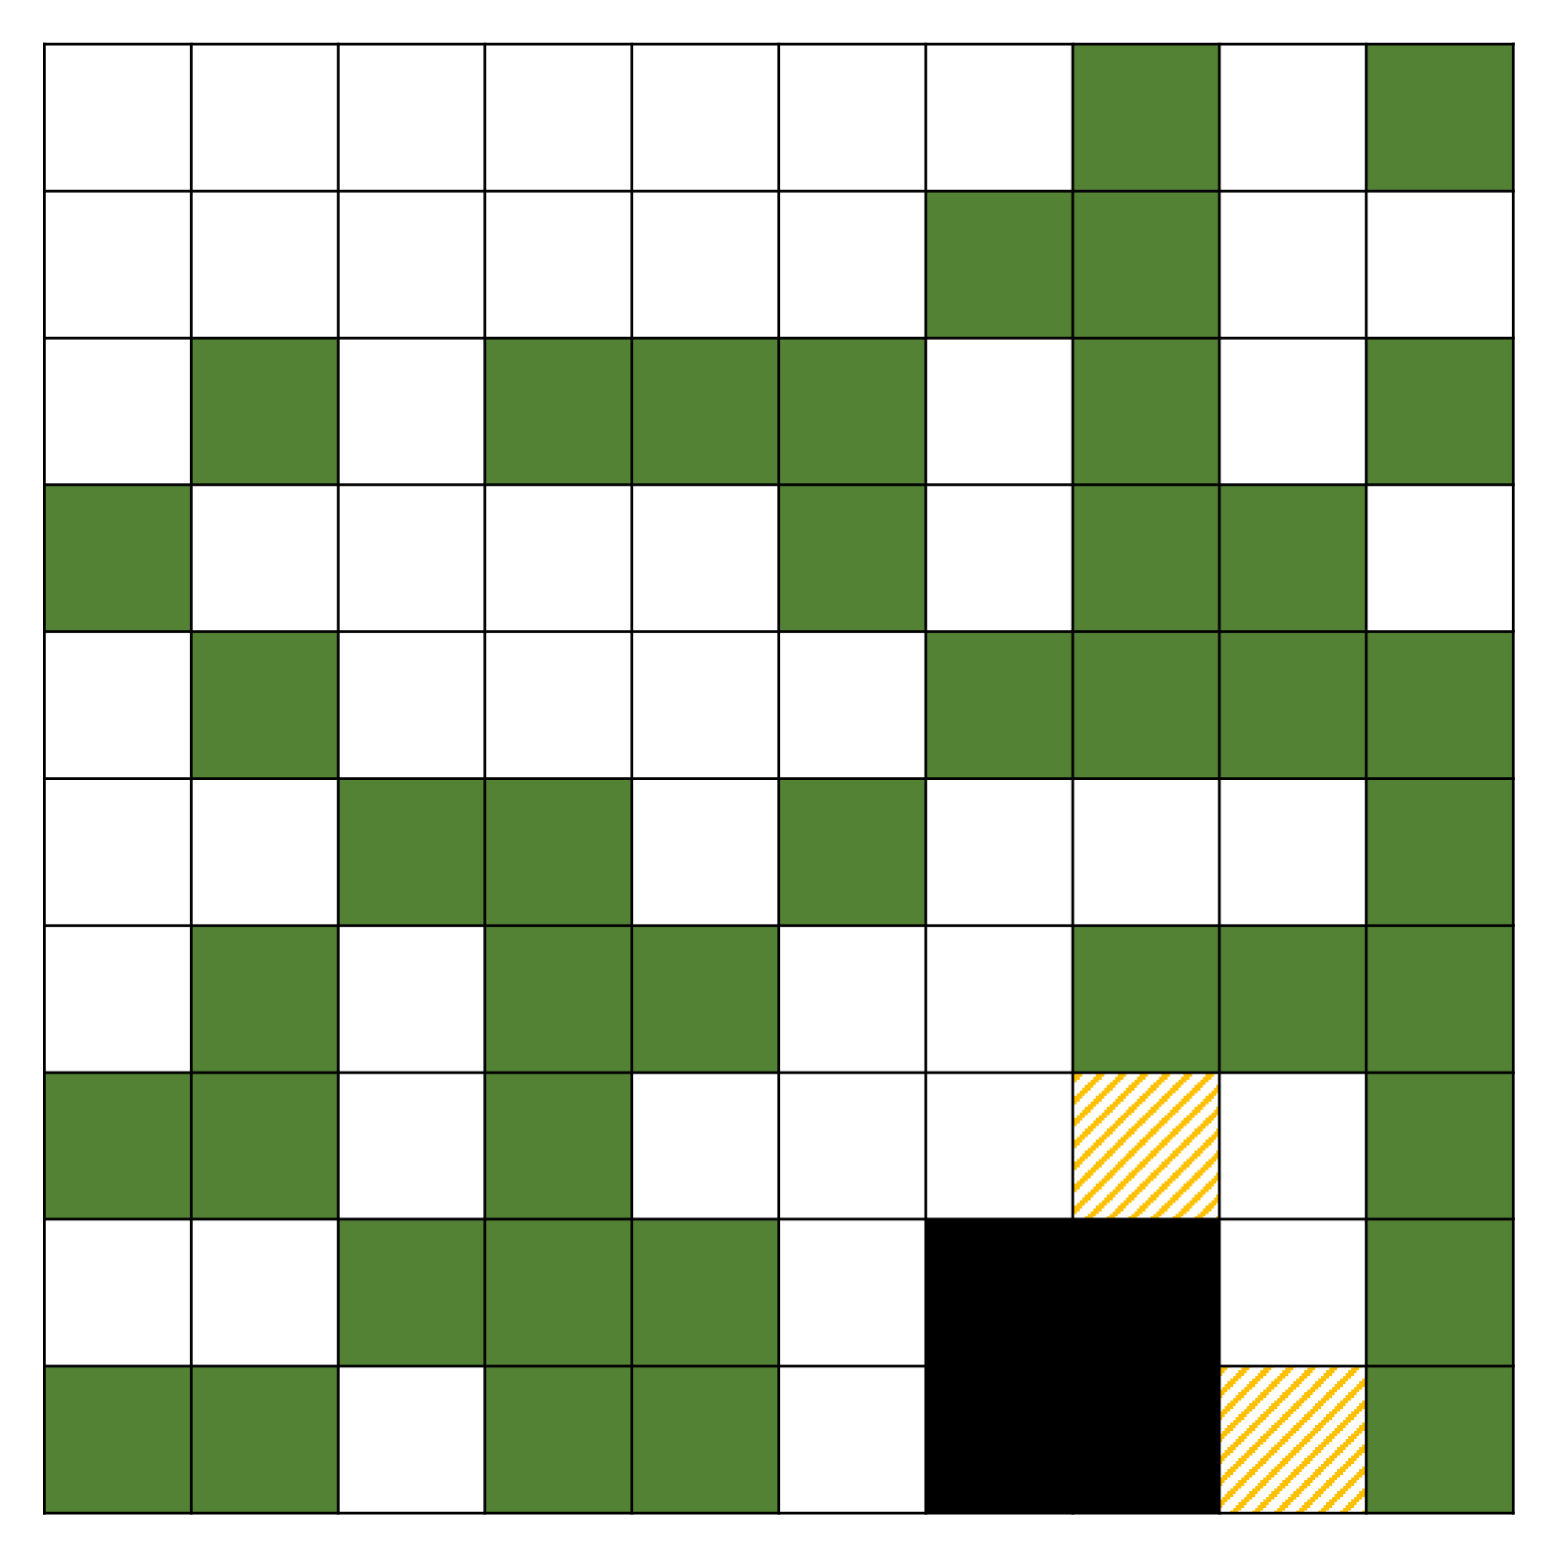
\includegraphics[width=0.4\linewidth]{firebreak/defended/end} 
%    \caption{End of outbreak ($t=3$)} 
%    \label{fig:end_defended} 
%  \end{subfigure} 
%  \caption{Outbreak of fire on a defended percolated graph}
%  \label{fig:percolated_defended} 
%  \end{centering}
%\end{figure}
%
%If, for instance, we could only remove two vertices as a firebreak, we ought to make those two the ones shown in yellow in figure \ref{fig:percolated_defended}. This is an example of how percolating a graph for use in {\scshape Firefighter} (and indeed {\scshape Firebreak}) can assist in generating a more realistic and useful model for contagion. There is much interest in the regular graph examples, but our modelling contexts of interest call for a more sporadic graph density and so we, in future research, will try and prove conjectures regarding the minimum number of vertex defences required in {\scshape Firebreak} for percolated graphs of given percolation threshold and dimension (or infinite graphs) and analogous questions in {\scshape Firefighter}.
%
%These random graphs are very reminiscent of Erd\"{o}s R\'{e}nyi random graphs and this is for good reason. In fact, the Erd\"{o}s R\'{e}nyi process of graph generation - adding edges into a graph with some given probability $p$ - can be thought of as bond percolation on the complete graph with probability $1-p$.

\end{document}